\section{Redes Neurais}
\label{s.neural_networks}

\subsection{Neurônios e o Cérebro}

Nesta seção, vamos discutir sobre os princípios das redes neurais. Tais técnicas tentam imitar o cérebro humano, sendo vastamente utilizadas nas décadas de 80 e 90. Com o surgimento de novas ferramentas por volta do meio da década de 90, sua popularidade acabou por decrescer. Entretanto, elas voltaram a ter um foco maior devido às abordagens baseadas em aprendizado em profundidade. Segue um exemplo de um simples neurônio:

\begin{figure}[!h]
\centering
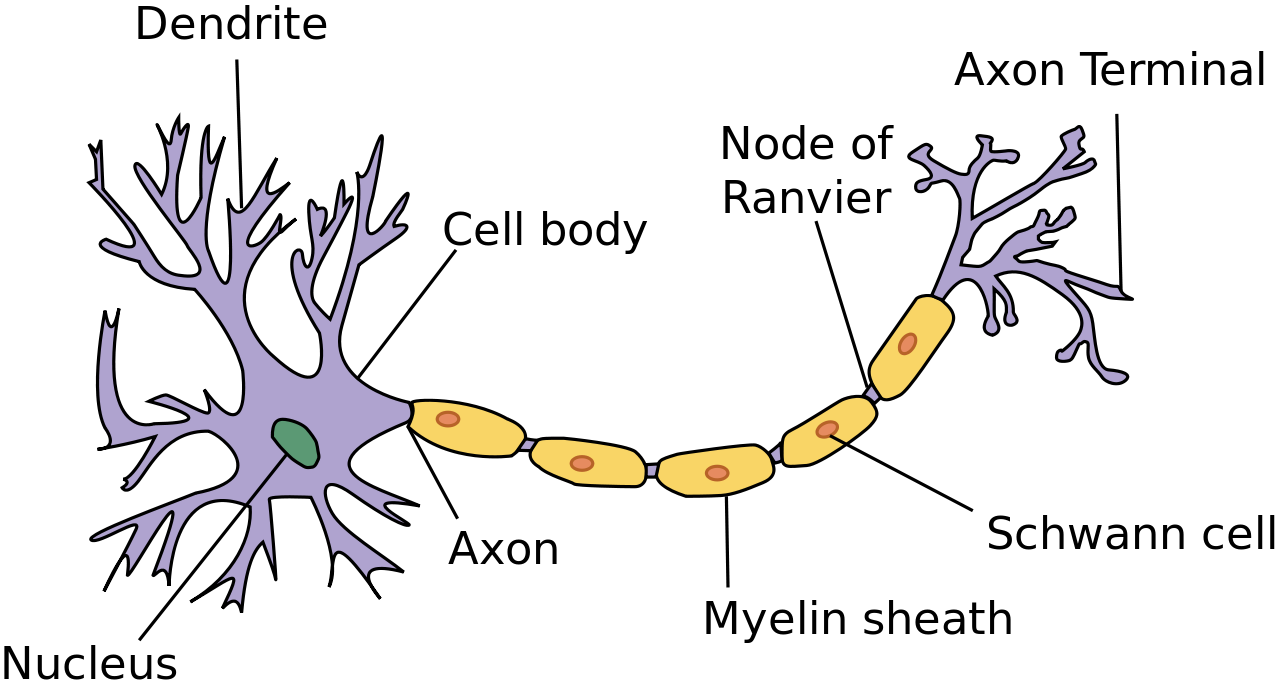
\includegraphics[scale=0.25]{figs/neuron.png}
\label{f.neuron}
\end{figure}

Basicamente, os neurônios comunicam entre si por meio da emissão de pulsos elétricos a partir de suas entradas (dendrito) para suas saídas (axônio). Matematicamente falando, podemos representar um simples neurônio como segue:

\begin{figure}[!h]
\centering
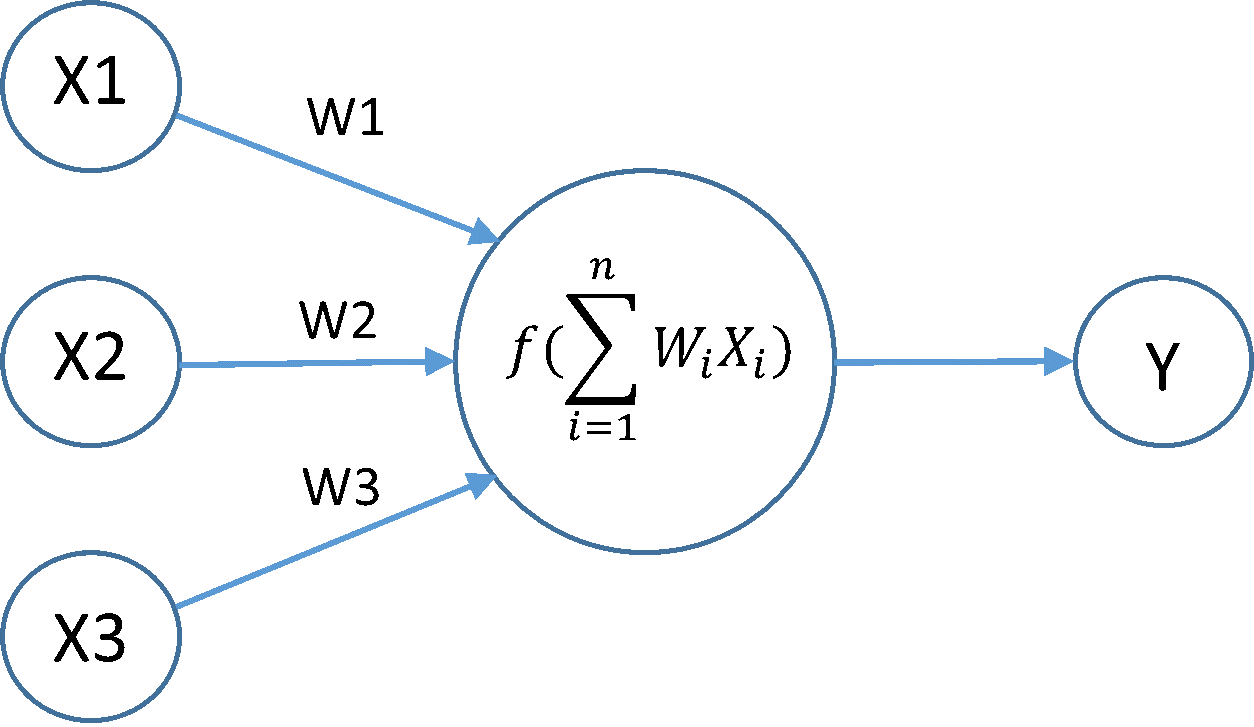
\includegraphics[scale=0.30]{figs/simple_neural_network.png}
\label{f.simples_neural_network}
\end{figure}

Uma \textbf{função de ativação} comum que pode ser utilizada é:

\begin{equation}
\label{e.activation_function}
g(z) = \frac{1}{1 + e^{-z}}, \text{onde} \ z = w^Tx	
\end{equation}

ou uma função limiar:

\begin{equation}
\label{e.limiar_function}
g(z) =
   \begin{cases}
      1, & \text{if}\ z \geq \theta \\
      0, & \text{se}\ z < \theta,
    \end{cases}
\end{equation}

onde $\theta$ é um limite dado.

A equação acima pode ser reescrita como segue:

\begin{equation}
\label{e.limiar_function_r}
h_w(x) =
   \begin{cases}
      1, & \text{se}\ w^Tx \geq \theta \\
      0, & \text{se}\ w^Tx < \theta.
    \end{cases}
\end{equation}

\subsection{Perceptron}
\label{ss.perceptron}

O Perceptron foi proposto formalmente por McCulloch e Pitts em 1943 com o intuito de modelar um neurônio biológico. Entretanto, ele possui uma capacidade limitada em termos de poder discriminativo, dado que ele é capaz de aprender apenas um único hiperplano.

Novamente, vamos considerar nosso conjunto de treinamento $X = \{(x_0, y_0), (x_1, y_1), \dots, (x_n, y_n)\}$, onde $x_i \in \mathbb{R}$ e $y_i \in \{0, 1\}$. Para uma dada amostra $x \in X$, temos a seguinte situação:

\begin{table}[h]
\centering
\begin{tabular}{c|c|c}
\hline
\textbf{\small Rótulo Verdadeiro $(y)$} & \textbf{\small Rótulo Proposto $h_w(x)$} & \textbf{Erro} $\epsilon$\\\hline \hline
{\small 0} & {\small 0} & {\small 0}\\\hline
{\small 1} & {\small 0} & {\small 1}\\\hline
{\small 0} & {\small 1} & {\small -1}\\\hline
{\small 1} & {\small 1} & {\small 0}\\\hline
\end{tabular}
\label{t.perceptron}
\end{table}

Podemos reescrever a função de ativação limiar como segue:

\begin{equation}
\label{e.limiar_function_r1}
h_w(x) =
   \begin{cases}
      1, & \text{se}\ w^Tx - \theta \geq 0 \\
      0, & \text{se}\ w^Tx  - \theta < 0.
    \end{cases}
\end{equation}

Se considerarmos $w_0 = -\theta$, então temos:

\begin{equation}
\label{e.limiar_function_r2}
h_w(x) =
   \begin{cases}
      1, & \text{se}\ w^Tx \geq 0 \\
      0, & \text{se}\ w^Tx < 0.
    \end{cases}
\end{equation}

Antes de aprender o mecanismo de funcionamento do Perceptron, temos que compreender alguns conceitos relacionados à projeções e produtos internos. Suponha que tenhamos dois vetores $w = [w_1 w_2]$ e $x = [x1 x2]$. Podemos definir o seu produto interno (vetorial) entre $w$ e $x$ como: $w^Tx$. Podemos visualizar tal ideia como segue:

\begin{equation}
\parallel w \parallel = \sqrt{w_i^2 + w_2^2} \in \mathbb{R} \Rightarrow \text{tamanho (norma) do vetor} \ w	
\end{equation}

E o produto interno pode ser representado como segue:

\begin{center}
$p =$ tamanho da projeção de $w$ em $x$.
\end{center}

Portanto, $w^Tx = p \parallel w \parallel$.\\

Consideremos a situação onde $y = 1$ e $h_w(x) = 0$. Neste caso, $\epsilon = (y - h_w(x)) = (1 - 0) = 1$ (erro). Dado $h_w(x) = 0$, então temos que $w^Tx < 0$ (função de ativação limiar).

Também temos que $w^Tx < 0$ significa $p \parallel w \parallel \Rightarrow p < 0$. Entretanto, necessitamos $h_w(x) = 1$ para acertar a classificação. A fim de se obter isto, é desejável mover $w^{(t)}$ em direção à $x$, onde $w^{(t)}$ significa o valor de $w$ na iteração $t$.

Nesta situação, podemos obter $w^{(t + 1)}$ como segue: $w^{(t + 1)} = w^{(t)} + \eta x$, onde $\eta$ é a taxa de aprendizado.

Agora, suponha outra situação, onde $y = 0$ e $h_w(x) = 1$. Neste caso, temos que $\epsilon = (y - h_w(x)) = (0 - 1) = -1$ (erro). Portanto, temos que $w^Tx \geq 0$, mas necessitamos $w^Tx < 0$ dado que $y = 0$.

Portanto, podemos computar $w^{(t + 1)}$ como segue: $w^{(t + 1)} = w^{(t)} - \eta x$. Podemos juntar as duas equações em somente uma:

\begin{equation}
w^{(t + 1)} = w^{(t)} + \eta \epsilon x, \text{onde} \ \epsilon \in \{-1, 0, 1\}.
\end{equation}\\

Finalmente, o algoritmo de treinamento do perceptron é dado como segue:

\begin{enumerate}
\item Inicializar $\eta$;
\item Inicializar $w$ (pesos aleatórios);
\item Aplicar $w^{(t + 1)} = w^{(t)} + \eta \epsilon_i x_i, \forall i = 1, 2, \dots, m$ e $\epsilon_i(y_i - h_w(x+i))$;
\item Repetir passo (3) até que $\epsilon_i = 0$ para todos os elementos em $X$.
\end{enumerate}

\subsection{Perceptron Multi-camadas}
\label{ss.multi_perceptron}

Uma rede neural é basicamente um grupo de neurônios, como segue:

\begin{figure}[!h]
\centering
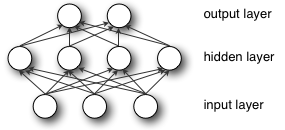
\includegraphics[scale=0.75]{figs/mlp.png}
\label{f.mlp}
\end{figure}

Considerando a rede acima, temos:

\begin{center}
$a_1^{(2)} = g(w_{01}^{(1)} x_0 + w_{11}^{(1)} x_1 + \dots + w_{n1} x^n)$
\\~\\
$a_2^{(2)} = g(w_{02}^{(1)} x_0 + w_{12}^{(1)} x_1 + \dots + w_{n2} x^n)$
\\~\\
$h_w(x) = a_1^{(3)} = g(w_{01}^{(2)} a_0^{(2)} + w_{11}^{(1)} a_1^{(2)} + w_{21}^{(2)} a_2^{(2)})$
\end{center}

Podemos também representar a rede neural como uma matriz de elementos como segue:

\[X=
  \begin{bmatrix}
    x^0 \\
    x^1 \\
    x^2 \\
    \vdots \\
    x^n
  \end{bmatrix}\]
  
\[Z^{(2)}=
  \begin{bmatrix}
    z_0^{(2)} \\
    z_1^{(2)} \\
    z_2^{(2)} \\
  \end{bmatrix} = (w^{(1)})^T X\]
  
\begin{center}
$a^{(2)} = g(z^{(2)} \Rightarrow h_w(x) = a^{(3)} = g(z^{(3)}$
\\~\\
$z^{(3)} = (w^{(2)})^Ta^{(2)}$
\end{center}

$Z_i^{(k)}$ refere-se aos dados de entrada do neurônio $i$ da camada $k$. Note que o processo computacional das ativações das unidades de entrada, escondida e saída é chamado de \emph{forward propagation}.

Se tivermos um problema de classificação de múltiplas classes, então o número de saída de neurônios será o mesmo que o número de classes.

Suponha que tenhamos um problema com $3$ classes. Portanto, $h_w(x) \in \mathbb{R}$. Considerando o problema, cada unidade de saída é composta por 3 classificadores de regressão logística.

\subsection{Parâmetros de Aprendizado}
\label{ss.learning_parameters}

Agora, a próxima questão é: como podemos aprender o conjunto de parâmetros $w = (w^{(1)}, w^{(2)}, \dots, w^{(L-1)})$, onde $L$ é o número de camadas. Seja $s_l$ o número de neurônios na camada $l$ (não estamos considerando as unidades de \emph{bias}).

Vamos rever a função de custo utilizada pela Regressão Logística.

\begin{equation}
\label{e.nn_costfunction}
J(w) = \frac{1}{m}[\sum\limits_{i=1}^m (y_i log(h_w(x_i)) + (1 - y_i) log(1 - h_w(x_i)))] + \frac{\lambda}{2m}\sum\limits_{j=1}^m w_j^2	
\end{equation}

Considerando uma rede neural com $k$ classes, então teremos $k$ classificadores de regressão logística na unidade de saída. Portanto, a função de custo deve considerar esses $k$ classificadores logísticos, como uma generalização da Equação~\ref{e.nn_costfunction}:

\begin{equation}
J(w) = \frac{-1}{m}[\sum\limits_{i=1}^m\sum\limits_{k=1}^k y_i^k log(h_w^k(x_i))+(1-y^k)log(1-h_w^k(x_i))] + \frac{\lambda}{2m}\sum\limits_{l=1}^{L-1}\sum\limits_{i=1}^{s_l}\sum\limits_{j=1}^{s_{l+1}}(w_{ij}^{(l)})^2
\end{equation}

Nosso próximo passo consiste em utilizar um conhecido algoritmo para o aprendizado de parâmetros em redes neurais chamado de \emph{Backpropagation}. Basicamente, queremos minimizar $J(w)$, e para tal propósito necessitamos computar as derivadas parciais $\frac{\partial J(w)}{\partial w_{ij}^{(l)}}$, onde $w_{ij}^{(0)} \in \mathbb{R}$.

Suponha que tenhamos apenas uma amostra de treinamento $(x, y)$ e a seguinte arquitetura de rede neural:

Os passos da \emph{forward propagation} são dados como segue:

\begin{itemize}
\item $a^{(1)} = x$
\item $z^{(2)} = (w^{(1)})^T a^{(1)}$
\item $a^{(2)} = g(z^{(2)})$
\item $z^{(3)} = (w^{(2)})^T a^{(2)}$
\item $a^{(3)} = g(z^{(3)})$
\item $z^{(4)} = (w^{(3)})^T a^{(3)}$
\item $a^{(4)} = h_w(x) = g(z^{(3)})$	
\end{itemize}

O propósito do algoritmo do \emph{Backpropagation} é relacionado ao cálculo do gradiente. Temos uma nova variável $\iota_j^{(l)}$ que significado o erro do nó $j$ na camada $l$.

Considerando a rede acima, temos que:

\begin{itemize}
\item para cada camada de saída $(l = 4)$: $\iota_j^{(4)} = a_j^{(4)} - y_j \Rightarrow \iota^{(4)} = a^{(4)} - y$	
\item para cada camada escondida $l \in \{2,3\}$:
	\begin{center}
	$\iota^{(3)} = (w^{(3)})^T \iota^{(4)} \ast g^1(z^{(3)})$
	\\~\\
	$\iota^{(2)} = (w^{(2)})^T \iota^{(3)} \ast g^1(z^{(2)})$
	\\~\\
	$\iota^{(l)} = (w^{(l)})^T \iota^{(l+1)} \ast g^1(z^{(l)})$
	\\~\\
	$g^1 = $ derivada da função de ativação
	\end{center}
\end{itemize}

\textbf{Ex.:} $g(z^{(3)}) = a^{(3)}$, $g^1(z^{(3)}) = a^{(3)} \ast (1 - a^{(3)})$\\

O nome \emph{Backpropagation} refere-se ao fato de que são computadas $\iota^{(4)}$, $\iota^{(3)}$ e $\iota^{(2)}$, o que significa que retropropagamos o erro através da rede. Basicamente, as derivadas parciais são dadas por:

\begin{equation}
\frac{\partial J(w)}{\partial W_{ij}^{(l)}} = a_i^{(l)} \iota_j^{(l+1)}	
\end{equation}

Note que não estamos considerando o termo de regularização.






